\documentclass[11pt]{article}
\usepackage{natbib,har2nat}
\usepackage{xcolor,colortbl}
\usepackage{forloop}
\usepackage{graphicx}
\usepackage{pdfpages}
\usepackage{multirow}
\usepackage{outlines}
\usepackage{subcaption}
\usepackage[toc,page]{appendix}
\graphicspath{ {images/} }
\usepackage{geometry}
 \geometry{
 a4paper,
 total={170mm,257mm},
 left=20mm,
 top=20mm,
 }

\begin{document}

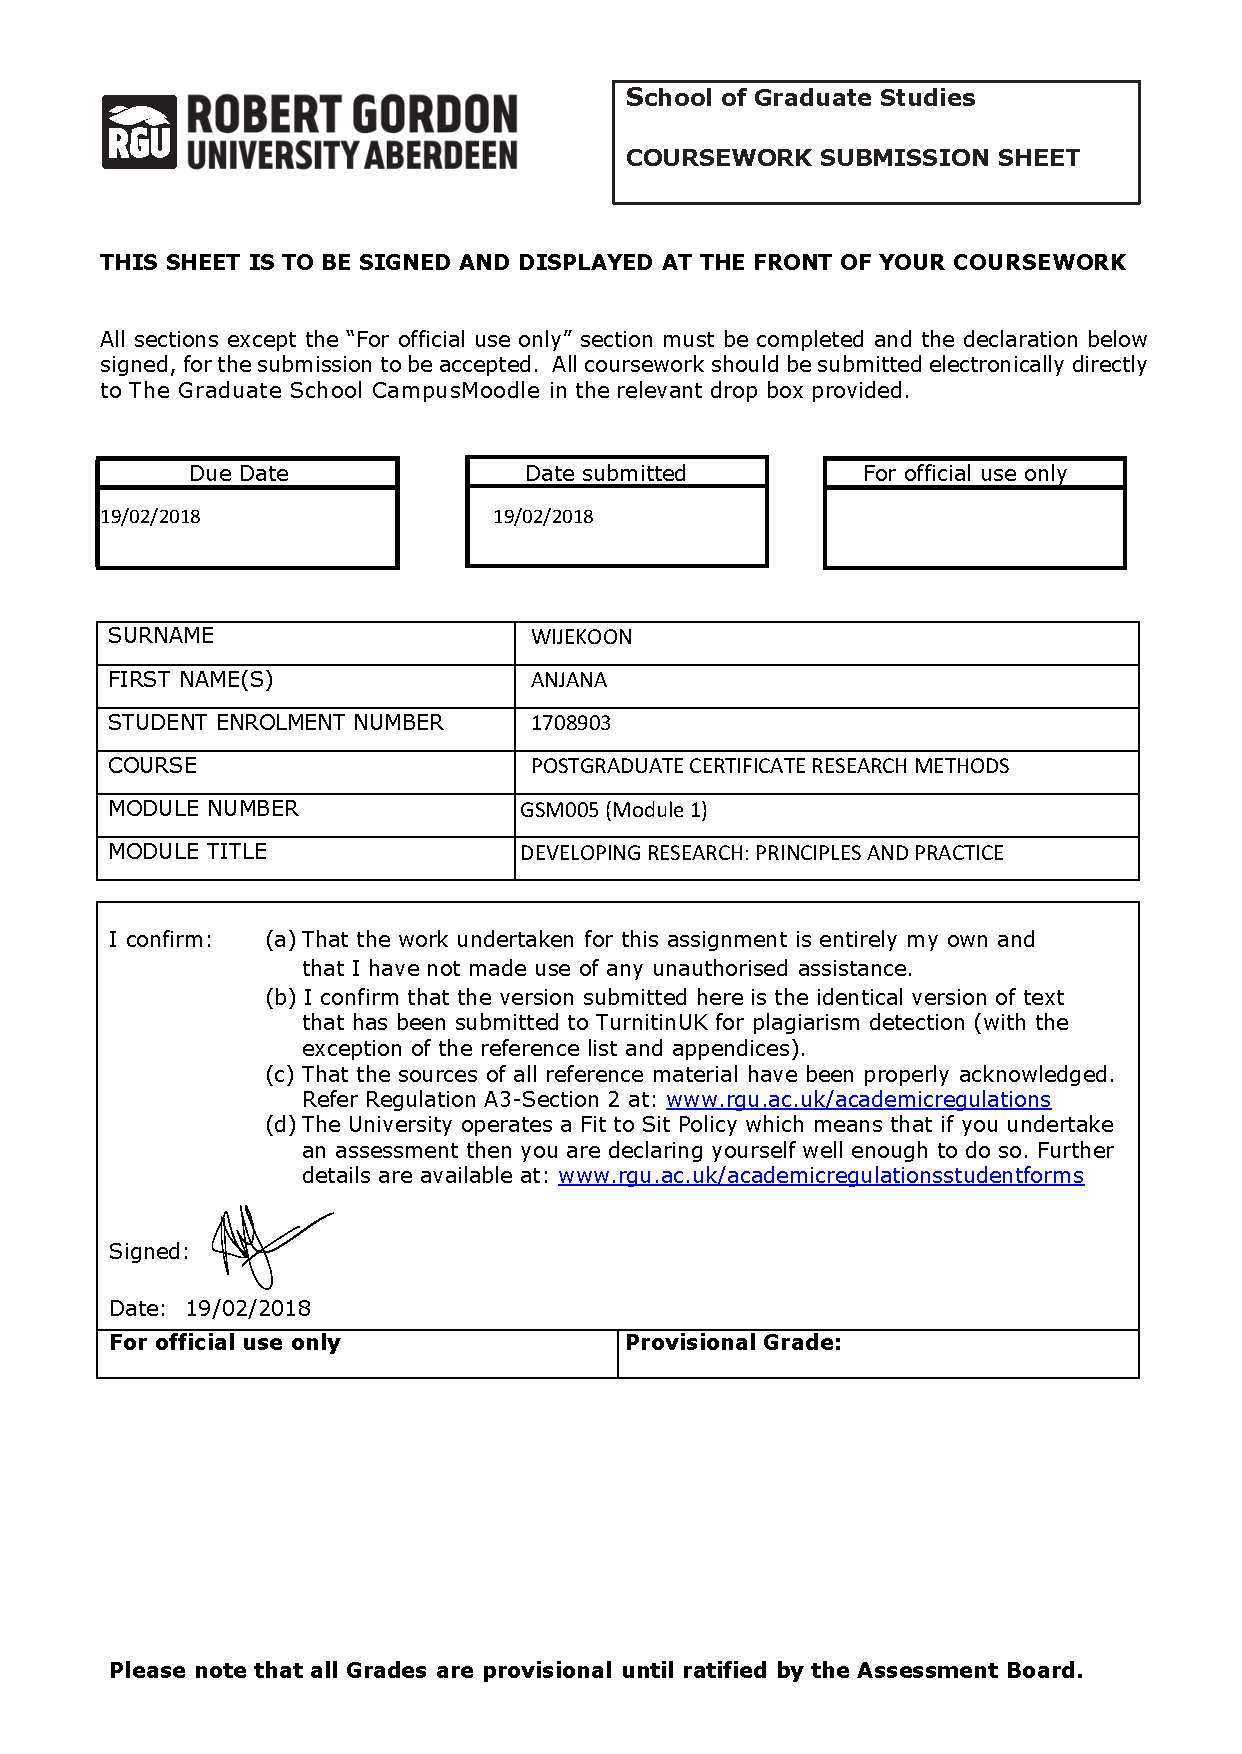
\includepdf{misc/cover.pdf}

\title{Reasoning with Multi-modal Sensor Stream Data for m-Health Applications}
\author{
Anjana Wijekoon (a.wijekoon@rgu.ac.uk) \\ 
Principle Supervisor: Prof. Nirmalie Wiratunga (n.wiratunga@rgu.ac.uk)}
\date{}
\maketitle 

\section*{Abstract}

Musculoskeletal Disorders (MSD) are chronic conditions which have a long term impact on individuals as well as on the community. They require self-management, typically in the form of maintaining an active lifestyle that adherence to prescribed exercises regimes. Therefore it is important to raise awareness about the importance of adherence and accordingly provide necessary support mechanisms to discourage sedentary lifestyles. In the recent past m-health applications gained popularity by gamification of physical activity monitoring and has had a positive impact on general health and well-being. However maintaining a regular exercise routine with correct execution needs more sophistication in human movement recognition compared to monitoring ambulatory activities (such as walking and running). In this research we propose a digital intervention which can intercept, recognize and evaluate exercises in real-time with a view to supporting exercise self-management plans. We will employ multiple sensors of different modalities (accelerometer, pressure and RGB+D sensors) to intercept exercises then implement reasoning methods to recognize and evaluate performance quality. We plan to compile a multi-sensor spatio-temporal dataset for exercises, then we will improve upon state of the art deep learning models to reason with that data. We expect our research contributions to be in the area of deep learning with focus on multi-sensor fusion algorithms and similarity comparison methodologies for spatio-temporal data. Importantly this work involves collaboration with the health sciences researchers to collect multi-modal exercise datasets which will be made public for comparative studies in human activity and exercise recognition research.

\section{Introduction}

Years lived with disability (YLD) is a measure of overall disease burden in a country and \citeasnoun{abajobir2017global} suggest one of the primary causes for YLD in developed countries is recognized as musculoskeletal disorders (MSDs). Maintaining a regular self-managed exercise routine is an essential component when living with MSDs. Specifically for elderly people (e.g. arthritis and hip-replacement) and many other chronic diseases (e.g. low-back pain, diabetes) it is important to maintain such routines and importantly to adhere to correct execution. Finding technological solutions to support either the prevention or self-management of MSDs has been a research area which has emerged over the last few years.

Trust in E-health digital interventions has grown in the healthcare community as increasingly effective methods are adopted with significant benefit realised in many disciplines (e.g. stroke prevention \cite{widmer2015digital}, self-management of asthma \cite{mclean2016interactive}, depression \cite{li2014game}). Digital interventions have also proven to encourage active lifestyle with the rise of smart devices \cite{fanning2012increasing}. For instance activity monitoring applications using smart devices collect data that help to keep track of user activities based on sensors that can be worn as well as those that are in the environment. For instance user activities such walking can now be captured through automated step counting with accelerometer sensors commonly found in mobile phones or watches. In contrast keeping track of exercises is completely relies on user input, resulting in poor accuracy and reliability. Therefore a digital intervention which captures exercises as they are performed and provides real-time feedback on performance quality would help to motivate the user to adhere to a regular exercise routine while supporting the collection of monitoring data crucial for the delivery of effective interventions.

An effective Digital intervention for self managing MSDs should consist of three main components: intercepting exercises in real-time to enable the automated data collection;  recognition of the exercise being performed; and the evaluation of the quality of the performance to facilitate personalised feedback generation. Today there are sophisticated sensors with improved sensing accuracy and efficient power consumption and they are the most recognized medium to intercepting human activities. Simple sensors on a smart phone are able to identify simple ambulatory activities. But an exercise is a sequence of independent movements of multiple body parts hence a smart watch on the wrist will not be able to capture an exercise with the level of precision required; furthermore a sensor is also likely to be susceptible to noise (due to a greater degree of freedom) not related to the exercise. Therefore it is evident that exercises require capturing different perspectives from multiple sensors, thus pose challenges of reasoning with multiple sensor modalities. 

Exercise recognition can be viewed as a special case of Human Activity Recognition (HAR). Research in this area involves the use of machine learning methods and more recently deep learning algorithms to reason with sensor data. \citeasnoun{yao2017deepsense} and \citeasnoun{hammerla2016deep} show that Convolutional Neural Networks, Recurrent Neural Networks and Deep hybrid architectures have been explored in this regard and yielded significantly better results when compared with traditional classification methods or Deep Neural Networks. We also explore the use of these architectures and our initial experiments (in Appendix \ref{appendix:selfback}) suggest that combining sensor modalities does not necessarily improve reasoning accuracy. Therefore it is important to explore sensor combinations and configurations to support improved reasoning with multi-modal data.  

In the rest of this document we will present literature in Section \ref{sec:literature} and then conclude with gaps that drive our research. Thereafter we propose research questions in Section \ref{sec:rq} and list expected outcomes in Section \ref{sec:outcomes} followed by proposed methods in Section \ref{sec:methods} to address our research questions. 

\section{Literature Review}
\label{sec:literature}
We discuss literature organised into several key elements; starting with an overview of the variety of sensors used for HAR; to different datasets that are available for model generation; analyse deep learning architectures; and paradigms suited to learning from multi-modal data streams. 

\subsection{Sensors}
\label{sec:sensors}
In the context of HAR, \citeasnoun{wang2017deep} lists three main modalities of sensors as body-worn , object and ambient sensors. Inertial sensors such as accelerometers and gyroscopes are examples of body worn sensors; whilst object sensors are those that are commonly mounted on an object to record movement or a sensor which observes a specific object. Here inertial sensors and cameras (RGBD/Depth) can be used as object sensors.Pressure sensors and temperature sensors are examples of ambient sensors where object/human interactions are sensed in a restricted area. For instance a surface can have many pressure sensor points which generate a sequence of heat-maps for pressure changes over time. Considering data generated by sensors, we can observe that wearable typically generate time-series data along several axes. For instance an accelerometer records acceleration of the subject along three axes. Sensors such as a pressure mats and depth cameras also generate time series data, but these are captured as images. 
When multi-modalities are used to capture sensor data synchronously in real-time (such as in bespoke hybrid sensors in smart home environments) the challenge for model learning is to generate data representations that enable the utilisation of all modalities and the effective fusion strategies to improve recognition accuracy for HAR.

\begin{table}
\caption{HAR datasets (A=Accelerometer, G=Gyroscope, M=Magnetometer, OS=Object Sensors, AS=Ambient Sensors, P=Pressure sensors) }
\label{table:data}
\begin{center}
\begin{tabular}{|c|c|c|c|c|} 
 \hline
 Dataset & Type & Subjects & Sensors & Classes \\
 \hline
 \citeasnoun{chen2015deep} & HAR &100 &A &8 \\
 \hline
 \citeasnoun{stisen2015smart} & HAR &9 &A and G &6 \\
 \hline
 \citeasnoun{bulling2014tutorial} & Gesture &2 &A and G &12 \\
 \hline
 \citeasnoun{chavarriaga2013opportunity} & ADL &4 &A, G, M, OS and AS &16\\
 \hline
 \citeasnoun{sundholm2014smart} & Sport Exercises &7 &P &10 \\
 \hline
\end{tabular}
\end{center}
\end{table}

Validation of HAR models in machine learning typically require datasets both for model generation and testing. Table \ref{table:data} summarises datasets used in recent HAR research. 
A notable difference is the dataset complied by \citeasnoun{chavarriaga2013opportunity} for Hierarchical Activity Inference (HAI), which allows the exploration of quality assessment applied to primitive action levels found in Activities of Daily Living (ADL). 
Unfortunately such primitives are not directly applicable for exercise recognition due to two reasons:
\begin{itemize}
\item sensor placements on limbs result in higher degrees of freedom and as such are not best placed to capture body movements in exercises as compared to ADL; 
\item the requirement for slower and controlled movement capture with exercises (certainly for MSDs) 
and the inherent characteristic of them consisting of longer sequences of sub-movements instead of shorter infrequent and non-repetitive movements as in ADL; and  
\item the need to capture greater floor surface with exercises further differentiates it from ADL calling for different types of sensing (e.g. pressure).  
\end{itemize}
When implementing reasoning models for sensing, these characteristics of exercises provide valuable insights that are not the focus of the the ADL dataset. Therefore in the context of multi-modal exercise recognition there is a clear need to capture and create new datasets to enable the advancement of exercise recognition research. 

\subsection{Deep Learning Models}
Advancement of computational power has enabled machine learning to evolve in to deep learning techniques. Deep learning models learn spatial and temporal dependencies in different abstraction levels given abundant data and has importantly eliminated the need for hand crafted features from raw data. Interestingly the model learning is closely coupled with the tuning of features that are being engineered. 

\subsubsection{Convolutional Neural Networks (CNNs)}\mbox{}\\
CNNs have demonstrated ability to learn spatial features and has been successfully applied in image classification, recommender systems and natural language processing. A convolution function extracts latent spatial dependencies in the input and organised in to feature maps. These feature maps can be viewed as creating new features through non-linear combinations of the raw input features. With increasing layers, extracted features enable the discovery of features that are increasingly conceptual in nature. 
Other aggregation operations are also included to generate layers, such as using the pooling functions, to reduce the spatial dimensions. Repeating these two operations provide feature embeddings in different abstraction levels providing the new features for classification or regression tasks (Figure \ref{fig:cnn}). 

\begin{figure}[ht]
\centering
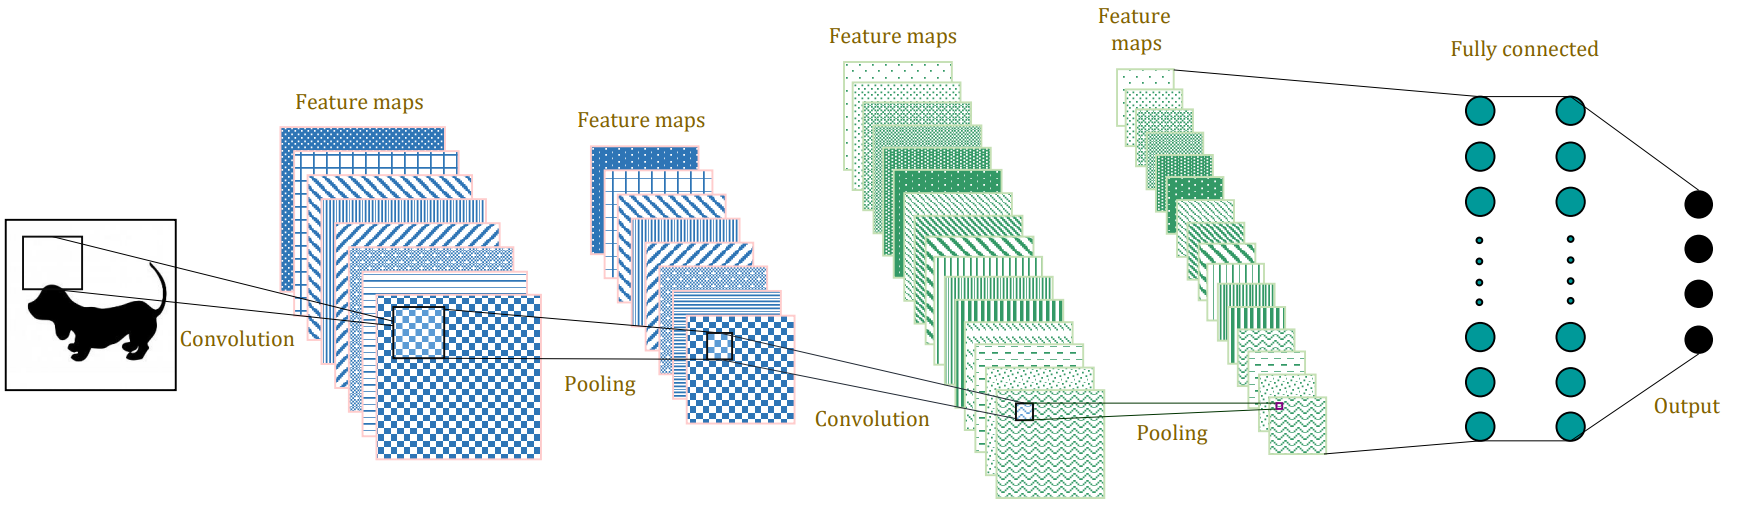
\includegraphics[width=0.8\textwidth]{cnn}
\caption{CNN with two convolution layers, second layer is a feature embedding used for the classification task}
\label{fig:cnn}
\end{figure}

\subsubsection{Recurrent Neural Networks (RNNs)} \mbox{}\\
RNNs learn dynamic temporal dependencies in data and have been applied successfully with time-series predictions, speech recognition and language translation. The Elman RNN cell (Figure \ref{fig:rnn}) is one of the basic implementations that demonstrate how RNN cell incorporates knowledge from previous time-stamp \cite{elman1990finding}. Unlike a CNN, this architecture focuses on retaining some memory of the recent learning session to influence the learning of the next iteration. Many advanced variations of RNN have been introduced since; such as LSTM, GRU and Bi-directional RNN \cite{chung2014empirical,schuster1997bidirectional}. 

Figure \ref{fig:rnn} illustrates the typical architecture of an RNN and the use of recurrence edges to introduce dependencies between time-stamps. With HAR data consisting of time dependant data, it makes sense to explore how these architectures compare with CNNs. Specifically we will explore whether the sophisticated convolutional feature embeddings can benefit from time dependant relationships that are discovered by RNNs.

\begin{figure}[ht]
\centering
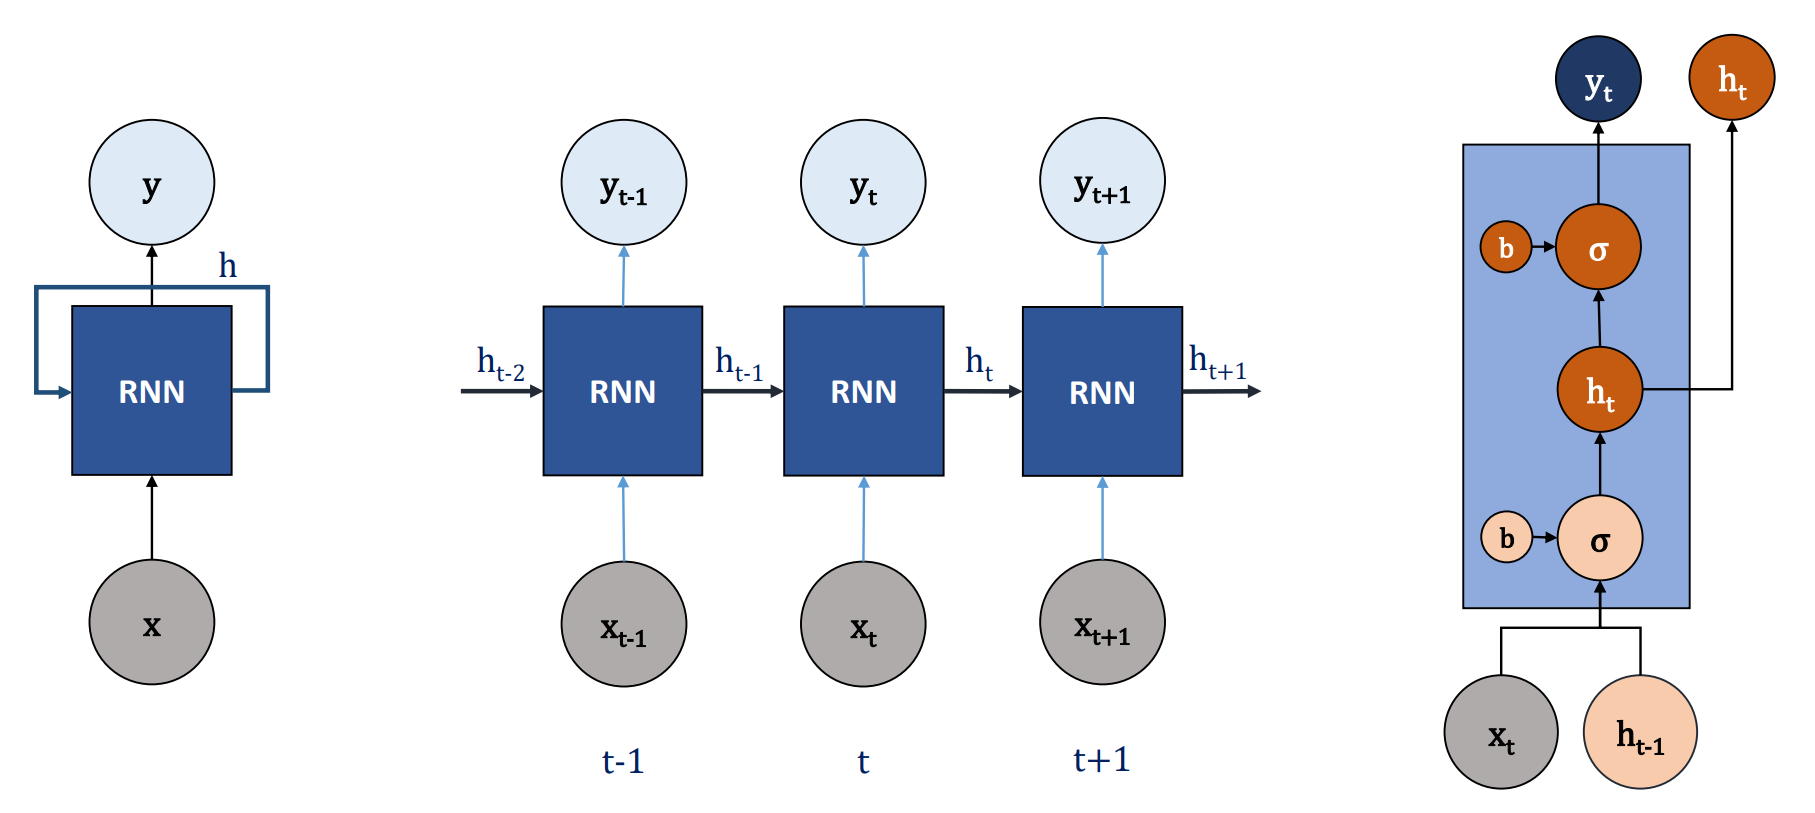
\includegraphics[width=0.7\textwidth]{rnn}
\caption{Recurrent Neural network, left: Simple RNN network, centre: RNN unfolding over time, right: Elman RNN cell}
\label{fig:rnn}
\end{figure} 

\subsubsection{Siamese Neural Networks (SNNs)} \mbox{}\\
\citeasnoun{chopra2005learning} introduced SNN as a neural network architecture that learn complex similarity metrics. Given two inputs, labelled as imposter or genuine, top layer of SNN generates a feature representation for each input that emphasises their similarity or dissimilarity. An interesting aspect of this architecture is that it enables the learning of metric space which in turn can be used to compare instances. \citeasnoun{chopra2005learning} employs SNNs for face verification tasks where CNNs build feature embeddings. We are interested in building comparable feature embeddings with spatio-temporal data from sensors which forms a novel application domain for SNNs.

\subsubsection{Auto-encoders} \mbox{}\\
\citeasnoun{hinton2006reducing} introduced the Auto-encoder (AE) as a multi-layer neural network with usually a single small central layer, where input is reconstructed at the output. The goal was to learn low-dimensional representation of the input data at the small central layer. First half of the network transforms input (encode) from high-dimensional data to low-dimensional encoding and second half of the network attempts to reconstruct data (decode) from low-dimensional encoding back to its original dimensionality. AE can be as simple as a shallow fully connected network or a complex CNN (Figure:\ref{fig:ae}) depending on the type of data being learnt by the model.
AE are known for learning from noisy data \cite{vincent2010stacked} where the network learns from noisy input and attempts to reconstruct a de-noised output. Ability of AE to rebuild an input is an interesting approach to synthesising sensor data given our requirement to operate robustly even in circumstances of absent sensors.

\begin{figure}[ht]
\centering
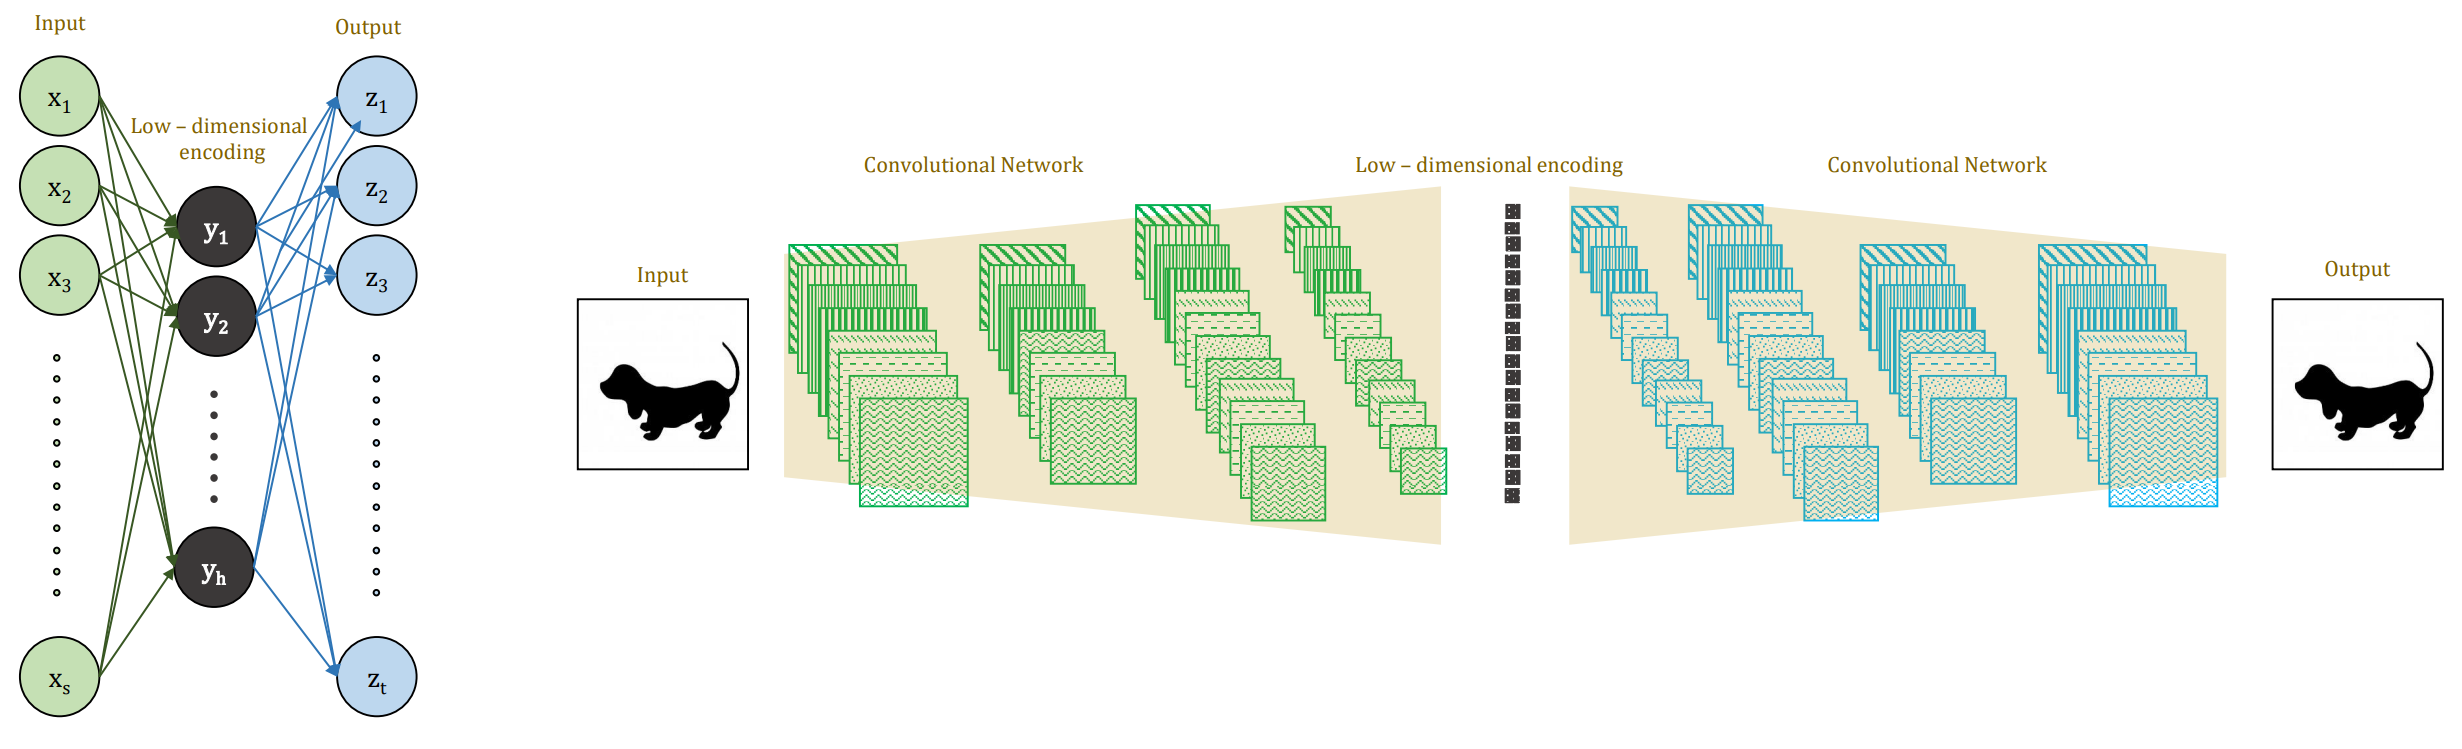
\includegraphics[width=1.0\textwidth]{autencoder}
\caption{Auto-encoders left: Shallow fully connected Auto-encoder, right: Deep Convolutional Auto-encoder }
\label{fig:ae}
\end{figure}

\subsection{Reasoning with sensors}

Early research suggests using machine learning models for activity classification needed feature engineering as a pre-processing stage. Features were extracted and refined from raw data using techniques such as Discrete Fourier Transform (DFT) and Principle Component Analysis (PCA). For instance \citeasnoun{garcia2011statistical} has used PCA to extract features from accelerometer and heart-rate data to perform Physical Activity Intensity classification; for a detailed discussion and comparative study of feature extraction methods the reader is refereed to \citeasnoun{preece2009comparison}. 

One of the main draw backs with employing hand-crafted features is that it requires several refinements using processes that are often decoupled from the model learning process. This often leads to features that remain domain specific where complex relationships are often not discovered making them less generalisable and transferable to new domains.

\subsubsection{Deep Learning Models in HAR}
The ability to engineer features as an integral part of model learning is a key advantage that deep learners have over traditional learning algorithms.
Specifically with time series data, 
\citeasnoun{ronao2016human} found that the input from two sensors can be used as different channels to the model. Their research shows that while CNN was seen to outperform traditional machine learning techniques with hand-crafted features, the hybrid approach of using temporal fast Fourier transform (tFFT) features with the CNN had resulted in the best performance. This research shows that hybrid approaches that combine both hand-crafted and learnt features lead to significant gains in HAR performance.

\citeasnoun{sani2017learning} is another notable research study involving accelerometer data from two body worn sensors on wrist and thigh. They implement a pyramid like CNN architecture in contrast to the inverted pyramid architecture from \citeasnoun{ronao2016human} which is the most common deep CNN silhouette. They compare how well each sensor captures the same activity and as expected found the thigh positioned accelerometer data to be robust with less noise for HAR tasks.

Together these studies provide important insight in to working with time series data with CNNs. They both adapt one dimensional convolutions to abstract temporal dependencies. Also from \citeasnoun{sani2017learning} results we can see that CNNs feature representation performs better when noise is present (wrist) compared to hand crafted features, when noise is less (thigh) there is no significant performance difference between hand crafted feature and CNN features. Therefore we can conclude that CNNs effectively abstracts desirable features in the presence of noise while learning temporal dependencies.

\citeasnoun{ordonez2016deep} presents an advancement to the previous architectures by adding recurrence to their architecture. They also treat multiple sensor inputs as channels to a single convolution architecture. In contrast to \citeasnoun{ronao2016human} they have an additional recurrence layer at the end of convolutional layers to learn temporal dependencies. Results show that raw time series data applied to their "DeepConvLSTM" outperformed both the vanilla CNN and other classification algorithms. In addition they show how using multiple sensor channels improve classification accuracy. But we can see the architecture is restricted and unable to fuse different modalities of sensor data. 

\citeasnoun{hammerla2016deep} explore different LSTM (Long Short Term Memory) architectures in HAR tasks. Their LSTM architectures were found to outperform a baseline CNN architecture on two of the three public datasets used in their study. They conclude that selecting the window size for chunking sensor input is crucial when working with LSTMs. Also repetitive activities such as walking or running favour CNNs over LSTMs compared to activities with natural ordering. This is an important insight when implementing deep models for exercises, because an exercise instance can be seen as consisting of both a natural ordering due to the expected sequence of body movements, as well as the repetitive nature of an exercise. Therefore we need to find the best balance between CNN and RNN components when designing a model for exercises. 

\subsubsection{Deep Sensor Fusion architectures}
Fusion architectures with deep models have been mainly investigated in the area of reasoning with video, where still images from video is treated as multiple inputs. \citeasnoun{karpathy2014large} and \citeasnoun{pigou2015beyond} use fusion architectures to classify video by experimenting fusion in different levels of abstraction. \citeasnoun{ngiam2011multimodal} using a RBM fusion architecture to reason with audio and video data. 
Unlike images or video stream, isolating related channels from time-series sensor data can be less obvious and must also consider similarity before they can be used together in this way. 
As discussed in Section \ref{sec:sensors} it is evident that a single sensor is not able to capture all human body movements specially for exercises, hence the need for multiple sensors. Research in sensor fusion is driven by this need and to expand models to exploit multiple sensors of different and complex data types. 

In the HAR domain \citeasnoun{radu2016towards} introduce a Random Boltzmann Machine(RBM) architecture for multi-sensor fusion. They use frequency domain features from two sensors; an accelerometer and gyroscope. This model has outperformed several shallow models with hand crafted features such as Decision trees (DT), Random Forest (RF) and Support Vector Machine (SVM). 

More recently \citeasnoun{yao2017deepsense} integrated  convolutional and recurrent architectures to learn spatial and temporal dependencies from multiple sensors. This "DeepSense" fusion architecture was evaluated for HAR with accelerometer and gyroscope data streams and was found to outperform Random Forests and SVMs with hand crafted feature. Thu also outperformed RMB and Multiple RBM architecture with frequency domain features from \citeasnoun{radu2016towards}.
\begin{figure}[ht]
\centering
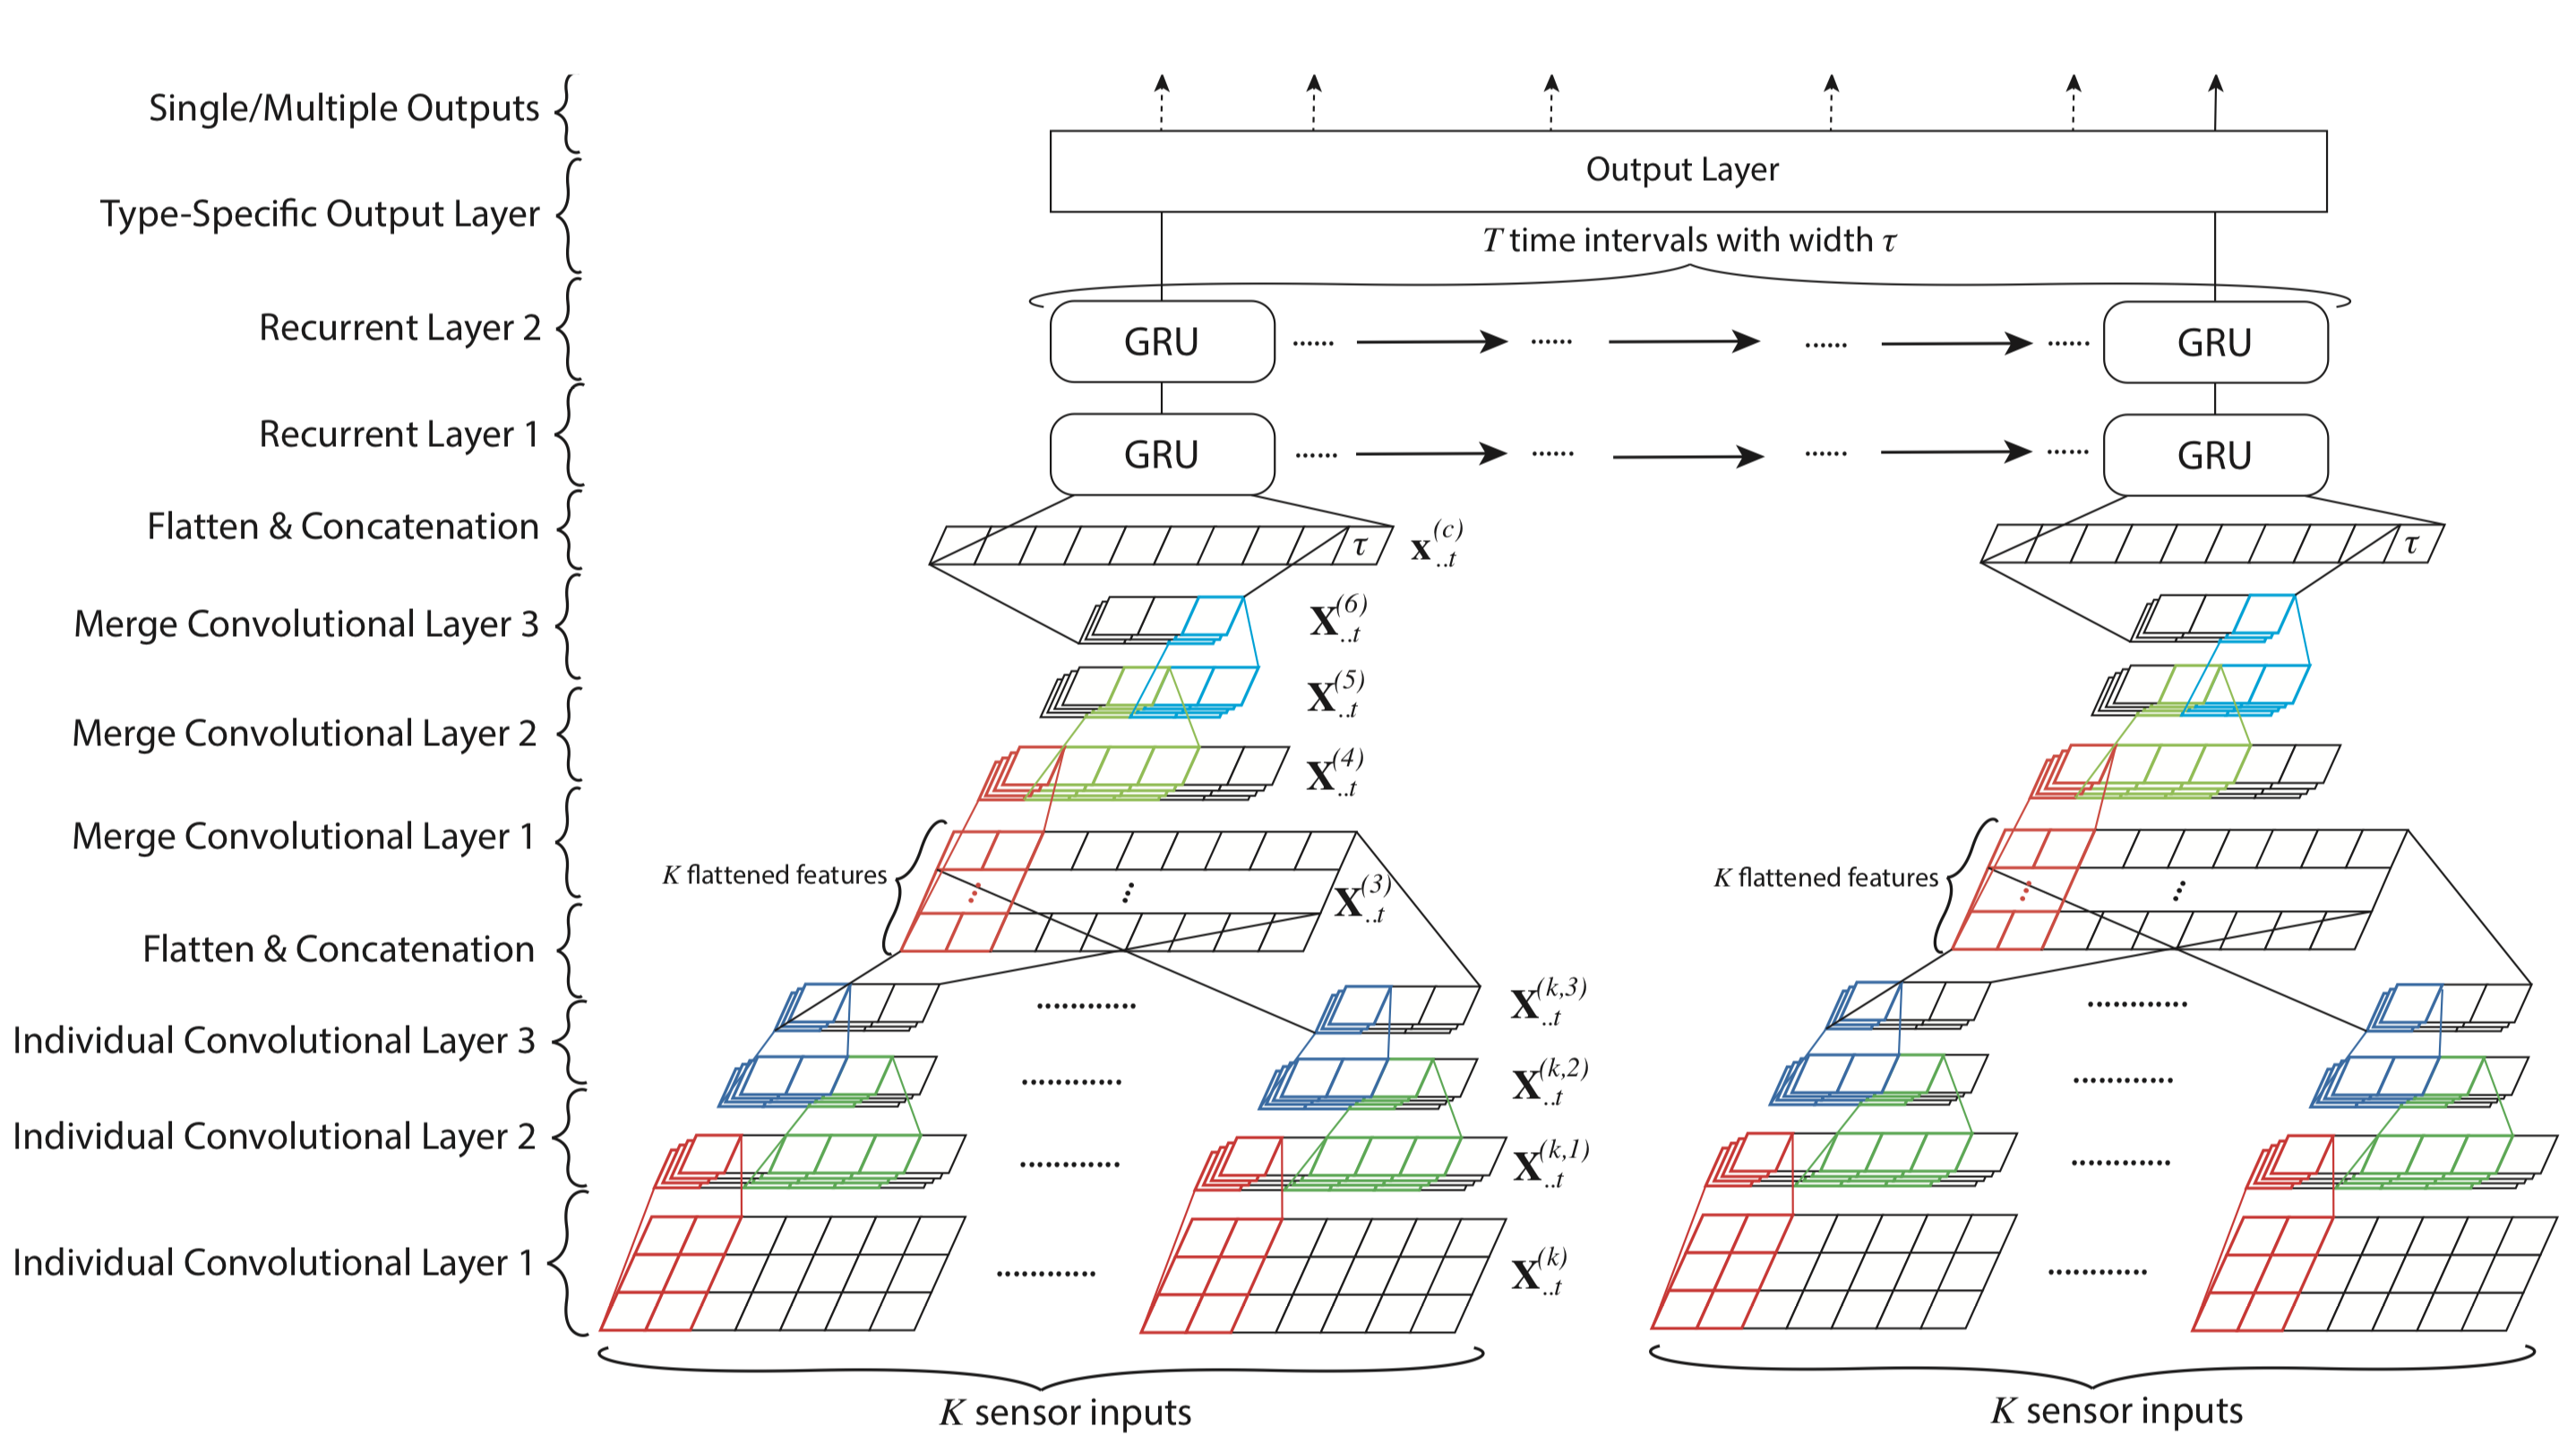
\includegraphics[width=0.6\textwidth]{deepsense}
\caption{DeepSense Architecture (\cite{yao2017deepsense})}
\label{fig:ds}
\end{figure}
A closer study of literature on sensor fusion architectures reveals that the evaluations however fail to present improvements that are statistical significant to support multiple sensors over a single sensor. In addition there is opportunity to improve on informed selection of sensors/features and noise reduction.  

\subsection{Attention}
Attention in deep models are mainly explored in the context of natural language processing but also seen in image processing to improve performance. 
They are a useful mechanism to optimise the manner in which features are attended upon for feature embedding.
In essence they provide a means to select features according to context as part of model learning.

\citeasnoun{mnih2014recurrent} introduce an attention mechanism with RNN to adaptively select regions from an input image or sequences from video. They mimic the human retina functionality by learning to focus on a selected region of the image. This selected area is learnt by the attention function, and the area outside this focus is considered as being blurred. Specifically the attention model is used to manage the area of of focus at input by updating the attention model based on feedback from the softmax output. 

Attention has also been applied with CNN architectures for Visual Question Answering tasks by ~\citeasnoun{chen2015abc}. Here unlike with RNNs the attention is used to influence the output from convolutions that are being learnt, by employing a number of convolution kernels on feature embeddings of an image to highlight the desired features for a given query embedding. This research interprets attention as selecting desirable convolution kernels per each query embedding and this approach outperforms the state of the art Bag-of-word methods and vanilla CNN or LSTM methods. 

In other related work attention has also been used to directly influence the the generation of the convolutional features~\cite{yin2015abcnn}. This provides an elegant means to influence one or more layers and has been successfully applied to NLP tasks to learn mutual influences between adjacent sentences for a given task. A Siamese Neural Net learns sentence similarities with a similarity-based attention matrix at each abstraction layer. Compared to \citeasnoun{chen2015abc}, this approach embed attention in to convolution layers. 

\subsection{Learning Paradigms}
In this section we detail three learning methodologies, each exploring different aspects of training machine learning models. We plan to explore these learning paradigms as needed in future in the context of  exercise classification and quality assessment. 

\subsubsection{Privileged Learning}
Privileged Learning (PL) mimics how humans learn with a teacher. In a learning environment teacher provides student with explanations, comments and examples but when tested student has to rely on what they learned. \citeasnoun{vapnik2009new} adapt this concept as an additional feature space (Privileged Information) that guarantees near perfect classification, but only available when the model is training. Defining Privileged Information (PI) is domain specific hence adaptable to many machine learning tasks.

\citeasnoun{chen2017training} use PI to minimize correlations between convolution functions. After learning feature representation for an input they suppress the background features using privileged knowledge, thus allowing the model to learn more foreground features desirable for classification. 

\citeasnoun{shi2017learning} attempt HAR with depth sequences for RNN with PI. Previous work involved with RNN and depth sequences required hand crafted features such as skeleton information which is a computationally expensive task. In this research they use Skeleton information as PI at training time and train a network for multiple tasks. First task is responsible for classification of depth sequence and second task learns to generate skeleton from depth sequence. At test time they use generated skeleton from the network itself as input for the classification task. 

Above literature exhibit that PI is open to interpretation. It enables building robustness in to models to handle missing modalities in real-time which improves usability and efficient deployment. 

\subsubsection{Sequence to Sequence Learning (\textit{seq2seq})}\mbox{}\\
Sequence to sequence Learning is an significant application domain of RNNs, specifically LSTMs. The goal is to generate a sequence from another sequence by learning inter-dependencies with LSTMs. Most notable and common usage is language translation where \citeasnoun{sutskever2014sequence} introduces \textit{seq2seq} with English to French translation. Improving on \cite{sutskever2014sequence}, \citeasnoun{luong2015multi} introduces multi-task \textit{seq2seq} learning where multiple encoders and multiple decoders learn multiple tasks in the same recurrence architecture. They evaluate language translation tasks in multi-task \textit{seq2seq} model.

We are interested in exploring \textit{seq2seq} in generating sensor data streams which does not appear in literature but interesting avenue to explore given their powerful ability to learn inter-dependencies and generate sequences. 

\subsubsection{Curriculum Learning}
Curriculum learning was first introduced by \citeasnoun{bengio2009curriculum} as defining a curriculum strategy for training a network. They adapt from human learning process where we start with simple examples and build up complexity. The curriculum strategy is open to interpretation decided by the application context.

\citeasnoun{havaei2016hemis} introduce a robust deep model to handle missing image modalities at test time by training the model with pseudo-curriculum training for medical imaging. All modalities were used as input in early epochs and then a random number of modalities were dropped from input for a given training instance enabling model to adapt to missing modalities. 

This methodology can be interpreted as a different perspective of PL as well where learning is interpreted as series of tests. 

\subsection{Exercise Quality}
Providing performance assessment is important in a digital intervention to maintain quality. but it is a subjective process. Performance quality of an exercise can be defined as how much actual execution deviates from correct execution of the exercise performed under the supervision of a physiotherapist. Measuring the deviation is open to interpretation and there is a lack of research in this area. Existing literature suggests performing classification on hand crafted features is the most explored method for determining quality of exercise. 

\citeasnoun{chen2013rehabilitation} is a notable publication on this area. Their data set consist of instances from both correct and incorrect performance of the exercises recorded with three accelerometers. Sensors were strategically placed on body to calculate angles of the body parts and with FFT features they classified type and correctness. In this research, correctness is modelled as binary classification task and provided in hindsight. 

\citeasnoun{velloso2013qualitative} model quality as a multi class classification task where one class represent correct execution while are different types of wrong executions. They also implement a rule based model where an execution will be matched against a set of rules derived from correct model. Rule-based approach out performs classification approach in their experiments and able to isolate the error to a single rule. 

Locating the problems within the sequence to provide meaningful feedback in real-time is a desirable feature in a qualitative evaluation and \citeasnoun{velloso2013qualitative} achieve with rule based system. But rule based system has many drawbacks such as need for expert knowledge, expense of maintenance and less generalizability. In addition above classification systems use hand crafted features and there is no evidence seen in literature exploring the advantages of deep models to address this task to our knowledge. 

\clearpage

\section{Research Questions and Objectives}
\label{sec:research_questions}
This research will explore reasoning with multiple sensors. The overall goal is to introduce novel components for a sustainable digital intervention for self-managing exercise routines. Following review of literature we identity research questions to achieve aforementioned goal . 

\paragraph*{Research Questions}
\label{sec:rq}
\begin{enumerate}
\item [RQ1] How to combine multi-modal data streams to improve exercise recognition?
\item [RQ2] How to maintain recognition accuracy in the presence of noisy and/or missing sensor modalities?
\item [RQ3] How to analyse exercise performance quality by comparing actual and expected multi-modal sensor data?
\end{enumerate}

\noindent We hope to meet following objectives in order to answer each research question. 

\paragraph*{Objectives}
\label{sec:outcomes}

\begin{itemize}
\item [O1] Compile a multi-modal sensor dataset in the domain of exercises with HAI using three sensing modalities. 

\item [O2] Develop a sensor fusion architecture with a dynamic attention layer to manage the combination of multi-modal sensor data to improve recognition accuracy. 

\item [O3] Implement methodologies to handle absence of modalities in real-time. 
This would enable the network to learn with all modalities but remain robust even with fewer modalities in real time. 

\item [O4] Introduce a similarity based architecture for comparing sensor data instances to generate a quality assessment. The resulting solution should localize performance problem to lower level actions of the exercise. 
\end{itemize}

\section{Proposed methodology}
\label{sec:methods}
In order to achieve our objectives we adopt and extend methods discussed in the literature review. These are explored further in the next sections.
\subsection{Objective 1}
Comprehensive multi modal sensor data collection for exercises is crucial if we are to address each research question mentioned above. As explored in the literature review, publicly available datasets for HAR and quality assessment seems to lack characteristics desirable to evaluate an end to end digital intervention. Therefore it is evident that there is a need for a dataset of multiple modalities with HAI for exercises. 
We propose a data collection task that will employ an array of sensor modalities with HAI.

\begin{figure}[ht]
\centering
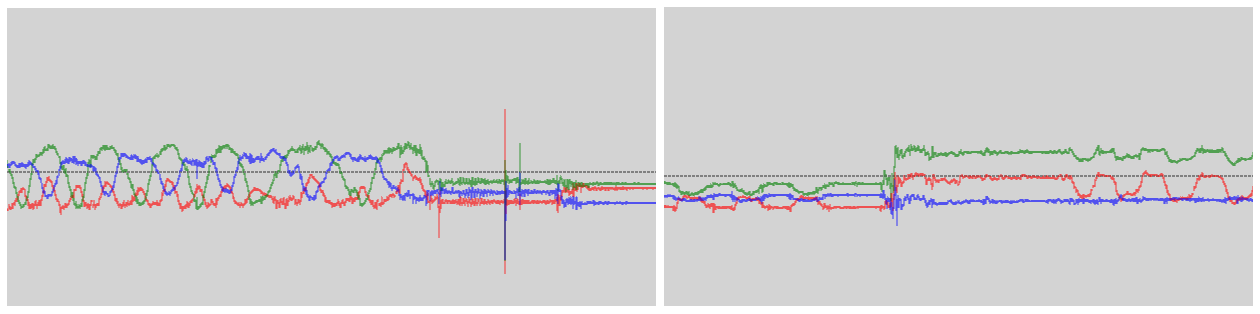
\includegraphics[width=0.8\textwidth]{acc}
\caption{Sample Accelerometer data}
\label {fig:acce}
\end{figure}

\begin{figure}[ht]
\centering
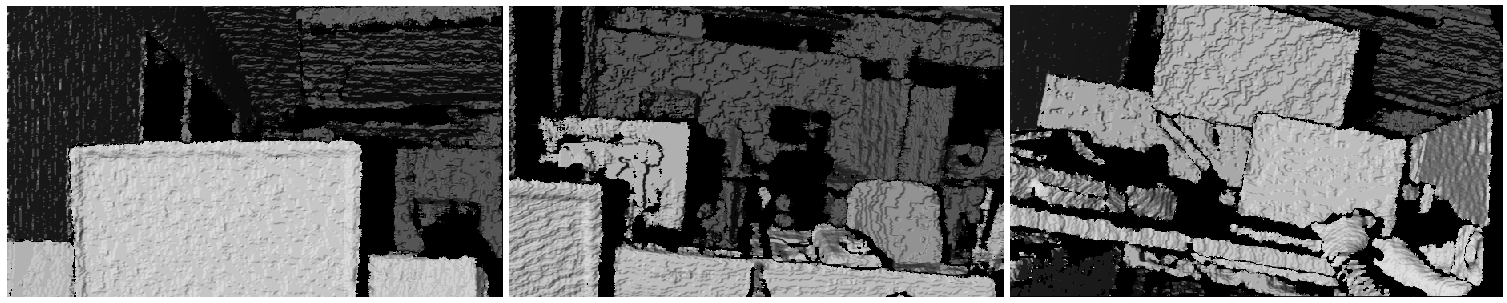
\includegraphics[width=0.8\textwidth]{dpt}
\caption{Sample Depth Camera data frames}
\label {fig:rgbd}
\end{figure}

Data collection will consist of two phases. First phase will focus on producing a multi-modal sensor dataset for exercise classification. We have selected accelerometers, pressure sensor and a depth sensor to bring together three different modalities. Figures \ref{fig:acce},\ref{fig:rgbd} and \ref{fig:pressure} show examples of these three modalities.

We have selected five exercises generally recommended for patients with low-back pain for this phase. Data will be recorded for thirty users each performing three sets of ten repetitions. A user will contribute roughly ten minutes of sensor data recordings and we will record approximately five hours of data distributed evenly across five classes. Data will be anonymized and analysed to remove outliers. This dataset will be used in design and evaluation of objectives 1 and 2.

\begin{figure}[ht]
\centering
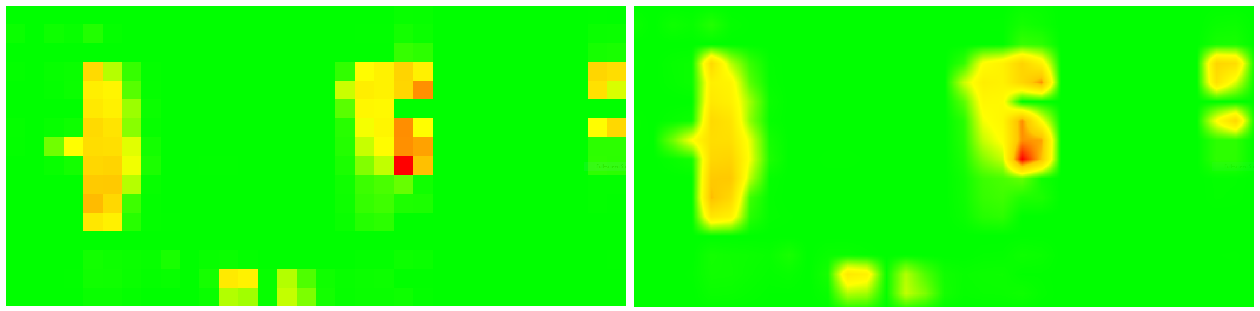
\includegraphics[width=0.8\textwidth]{pm}
\caption{Sample Pressure mat data frames, Left: Raw data frame (resolution 16x32), Right: Up-sampled with linear interpolation (resolution 512x1024) }
\label{fig:pressure}
\end{figure}

In phase two we will focus on producing a dataset with HAI by observing an exercise as a sequence of lower level actions. We will also create a test dataset with novice users to observe mistakes they do while performing the given exercises while labelling them on quality and on low level actions. The exercises and sensors selected for this phase will depend on conclusion we draw from objectives 1 and 2. 

\subsection{Objective 2}
To achieve objective 2 first we will investigate how each sensor modality contributes towards accurate classification of exercise movement classes and we will explore how a sensor fusion architecture can contribute toward improving previous results. Then we look at informed selection of sensors with an attention mechanism. Attention can be interpreted in different levels. First level is informed selection of subset of sensors for a given classification instance. At this level the goal is to select the best subset of sensors to intercept and recognise given an exercise. Second level is informed selection of features from abstract feature representations. We will generate feature embeddings at several abstract levels with a CNN for each modality and an attention mechanism focusing on the most desirable features from each sensor for the given classification instance. The goal is to attend to the most informative features from different sensors to improve exercise recognition.

\subsection{Objective 3}
Efficient deployment is an important characteristic in any health care digital interventions with direct impact on user acceptance. In this problem domain, the main restriction is the number of sensors. More sensors force the user in to a more restricted setting hence efficiency is negatively correlated to the number of sensors used. Being inspired by the PL paradigm we will explore two approaches to address objective 3. First is enforcing robustness in sensor fusion model to handle missing modalities. We will adapt the curriculum learning methodology to address this. We can define easy instances as instances where all modalities are present and hard instances as instances with some modalities missing and apply curriculum learning by introducing easy to hard instances in training phase. Second we will investigate how we can generate synthetic data to represent missing modalities at real time by adapting auto-encoders. At training auto-encoders can learn to generate sensor stream for each modality from other modalities, at test time auto encoder can be used to estimate the missing modality from existing. Thereafter the classifier will be presented with all modalities which will include both estimated and those actually present. We will conduct a comparative study to find the best approach. 

\subsection{Objective 4}
To address objective 4 we must define a metric to assess exercise performance quality.
Specifically the deviation between expected and actual performance will form the basis for this metric.
We will look at how deep models can learn differences in spatio-temporal data belonging to one classification class to evaluate quality difference. This will call for similarity measures in different abstract levels of feature embeddings. In order to locate differences in finer detail we will treat exercises as a sequence of primitive actions. Here the idea is to isolate the differences with respect to a primitive action rather than performing a binary evaluation. 

\subsection{Evaluation of Deep Models}
We will perform leave-one-user-out (LOUO) evaluation on deep models to evaluate model's ability to generalise across different users. Since qualitative assessment is largely user dependant, we will evaluate research question 3 with n-fold cross validation with personalized datasets. All deep architectures will be subjected to statistical significance test to evaluate how our methods compare with current state of the art.

\subsection{Dissemination}
Datasets will be published though UCI Machine Learning Repository \footnote{http://archive.ics.uci.edu/ml/index.php}. We will generate literature at each phase of the research and disseminate through conferences and workshops. All code will be made publicly available through git-hub \footnote{https://github.com}. We identify following deliverables for each objective listed in Section \ref{sec:research_questions}

\begin{outline}
\1 Objective 1 
\2 Phase 1 - Publish multi-modal exercises classification dataset.
\2 Phase 2 - Publish multi-modal HAI dataset for exercise quality evaluation 

\1 Objective 2 
\2 Publication on informed selection of sensors in fusion architectures for better performance.

\1 Objective 3 
\2 Publication on working with multi-modal fusion architecture in the absence of sensor modalities in real-time.

\1 Objective 4
\2 Publication on similarity comparison with deep architectures for spatio-temporal data

\2 Publication on exercise quality evaluation with HAI. 

\end{outline}

\section{Overview of ethical issues}
A multi-modal spatio-temporal data collection for exercise classification and quality assessment is one of the main outcomes of this project. Dataset will comprise of sensor data recorded for list of exercises performed by number of participants. Compiling such dataset involves ethical issues in data collection and distribution.

First there are ethical considerations regarding the participants of the data collection task. Following guidelines were set for participants to evaluate their eligibility and get their consent.
\begin{itemize}
\item Participants are selected from volunteers aged above 18 years. 
\item Each participant will complete Physical Activity Readiness Questionnaire (PAR-Q) which will evaluate their fitness to perform the list of exercises. 
\end{itemize}
Next there are medical concerns that may occur during data collection. We set following guidelines to mitigate such situations.
\begin{itemize}
\item Hypo-allergenic tape will be used to minimize the reaction to adhesive tape used to fix sensors. If reaction occurs the participant will be stopped and sensors will be removed, if reaction fail to settle participant will be advised to seek medical attention. 
\item Participant will be stopped if any discomfort occur during data collection, also will be advised to consult a health care practitioner if discomfort fail to settle. 
\end{itemize}
Lastly there are ethical consideration regarding the data storage and distribution. 
\begin{itemize}
\item During data collection, data will be stored in a secure RGU server with restricted access.
\item At the completion of data collection, data will be anonymized to remove all participant identification information.
\item Anonymized dataset will be made public with publications based on the dataset. 
\end{itemize}
Above measures were presented and approved by the School Research Review Group of School of Health Sciences (Appendix \ref{appendix:ethics}).

\section{Identified Impact}

This research will introduce new state of the art methodologies for reasoning with multi-modal sensor streams. Machine learning research has evolved rapidly with the introduction of deep learning techniques build upon the support of tremendous computational power. We plan to build upon current deep learning techniques on HAR, adapt and improve them for multi-modal sensor reasoning for exercises. With objective 1 we will bring together different machine learning data domains such as time series, images and video as we create a multi-modal spatio-temporal dataset. It will be adaptable to different application domains as well as future research in HAI. It will also contribute towards evaluating transfer learning capabilities of machine learning models. Objective 2 will introduce new attention mechanisms for sensor data selection in abstract levels and in objective 3 we will introduce strategies to improve robustness in deep learning architectures.Objective 4 will implement novel deep learning models for qualitative evaluation which involves similarity comparison of spatio-temporal data. 

From the healthcare application perspective this research will contribute towards a sustainable digital intervention for MSD prevention and self-management while raising awareness. MSD has directly affects the workforce of a country with sedentary lifestyles and as a result it has a major impact on economical and social status of the country. This digital intervention will enable the user to perform physiotherapist recommended exercises at home with supervision from the qualitative evaluation component. We plan to involve users in each step of this research and raise awareness. We will seek user feedback on the utility of the digital intervention to support, maintain and encourage an active lifestyle in the prevention and management of MSDs.



\section{Time Management Plan}

\newcounter{loopcntr}
\newcommand{\onblue}[1][1]{
  \forloop{loopcntr}{0}{\value{loopcntr}<#1}{&\cellcolor{blue}}
}
\newcommand{\onbluee}[1][1]{
  \forloop{loopcntr}{0}{\value{loopcntr}<#1}{&\cellcolor{bluee}}
}
\newcommand{\off}[1][1]{
  \forloop{loopcntr}{0}{\value{loopcntr}<#1}{&}
}
\definecolor{blue}{HTML}{002b80}
\definecolor{bluee}{HTML}{ccddff}

\noindent\begin{tabular}
{|p{0.54\textwidth}
!{\vrule width 0.4mm}p{0.01\textwidth}*{3}{|p{0.01\textwidth}}
!{\vrule width 0.4mm}p{0.01\textwidth}*{3}{|p{0.01\textwidth}}
!{\vrule width 0.4mm}p{0.01\textwidth}*{3}{|p{0.01\textwidth}}
|}

\hline
\textbf{Time Management Plan} 
& \multicolumn{4}{c!{\vrule width 0.4mm}}{Year 1} 
& \multicolumn{4}{c!{\vrule width 0.4mm}}{Year 2} 
& \multicolumn{4}{c!{\vrule width 0.4mm}}{Year 3} \\

\hline
Literature Review \onblue[2] \onbluee[8] \off[2] \\
\hline
\textbf{Objective 1 - \mbox{Phase 1}} & \multicolumn{12}{c|}{} \\
\hline
Ethics approval \off[1] \onblue[1] \off[10]\\
\hline
Sensor selection and pre-configuration \off[1] \onblue[1] \off[10]\\
\hline
Data collection \off[2] \onblue[1] \off[9]\\
\hline
Data cleansing, annotation for classification\off[2] \onblue[1] \off[9]\\
\hline
\textbf{Objective 1 - \mbox{Phase 2}} & \multicolumn{12}{c|}{} \\
\hline
Data collection \off[8] \onblue[1] \off[3]\\
\hline
Data cleansing, annotation for qualitative assessment \off[8] \onblue[1] \off[3]\\
\hline
\textbf{Objective 2} & \multicolumn{12}{c|}{} \\
\hline
Recognizing exercises with single and multiple modalities \off[3] \onblue[2] \off[7]\\
\hline
Building attention mechanism for informed sensor fusion \off[4] \onblue[2] \off[6]\\
\hline
\textbf{Objective 3} & \multicolumn{12}{c|}{} \\
\hline
Building CL algorithm to enforce robustness to fusion architecture to handle missing modalities \off[5] \onblue[2] \off[5]\\
\hline
Building architecture to synthesize missing modalities \off[5] \onblue[2] \off[5]\\
\hline
Integrate solutions with informed sensor fusion\off[6] \onblue[2] \off[4]\\
\hline
\textbf{Objective 4} & \multicolumn{12}{c|}{} \\
\hline
Build similarity based architecture for exercise comparison\off[9] \onblue[2] \off[1]\\
\hline
Extend similarity architecture to isolate performance error to primitive action within the exercise sequence \off[10] \onblue[2]\\
\hline
Implement feedback mechanism \off[10] \onblue[2]\\
\hline

\end{tabular}

\clearpage

\bibliographystyle{agsm}
\bibliography{references}
\clearpage

\begin{appendices}

\section{Sensor Fusion with SelfBACK}
\label{appendix:selfback}
SelfBACK HAR data set has been recorded by 34 users performing 6 activities while wearing accelerometer on wrist and accelerometer on thigh. Table \ref{table:dataset} is a summary of the dataset characteristics. The goal of this series of experiments is to find if accelerometer data from wrist and thigh can improve classification compared to wrist or thigh.

\begin{table}[ht]
\caption{SelfBACK HAR Dataset}
\label{table:dataset}
\begin{center}
\begin{tabular}{|c|c|} 
  \hline
  Number of users & 34 \\
  \hline
  Activities & Standing, Sitting, Walking, Upstairs, Downstairs, Jogging \\
  \hline
  Sensors & Accelerometers on wrist and thigh \\
  \hline
  Sampling rate & 100Hz \\
  \hline
\end{tabular}
\end{center}
\end{table}

\section*{Previous Work}
\label{sec:old}
Results from previous work on this dataset by \citeasnoun{sani2017learning} is summarised in Table \ref{table:results1}. Main conclusion we draw is that thigh accelerometer is a better source of data for HAR compared to wrist. High degree of freedom of wrist unrelated to the activity being performed contributes as noise and interfere with classification. 

\begin{table}[ht]
\caption{SelfBACK classification task with single sensor}
\label{table:results1}
\begin{center}
\begin{tabular}{|c|c|c|} 
  \hline
  \multirow{2}{*}{Classification task} & \multicolumn{2}{|c|}{F1 measure} \\\cline{2-3}
  & Wrist & Thigh \\
  \hline
  CNN-SVM & 0.850 & 0.957 \\
  \hline
  CNN-kNN & 0.845 & 0.949 \\
  \hline
  CNN & 0.839 & 0.959 \\
  \hline
  DCT-SVM & 0.836 & 0.967 \\
  \hline
\end{tabular}
\end{center}
\end{table}

\section*{Sensor Fusion}
\label{sec:fusion}
We conducted number of experiments to evaluate the effect of fusion between two accelerometer data from wrist and thigh. We used window size of 300 time stamps (3 second window) as input and performed Leave-one-user-out (LOUO) through out this series of experiments and present average accuracy from 34 experiments. We compare all experiments against the baselines of single sensor architectures. All our results are based on three layer convolution architecture for each individual CNN although figures show one convolution for clarity. Three layers are of 150, 100 and 60 feature maps maintaining consistency with the pyramid architecture introduced by \citeasnoun{sani2017learning}. These hyper-parameters were finalized after testing with different number of layer and number of feature maps.

First we explore fusion architectures to observe how fusion of these two sensor streams affect classification accuracy. Fist we learn feature embeddings of two sensors from individual CNNs, then fuse fuse feature embeddings with concatenation (concat) as two feature maps (Figure \ref{fig:concat}). Each input is shaped as one dimensional input of length 300 and three axis were used as 3 channels. Results are presented in Table \ref{table:fusion1}.

\begin{figure}[ht]
\centering
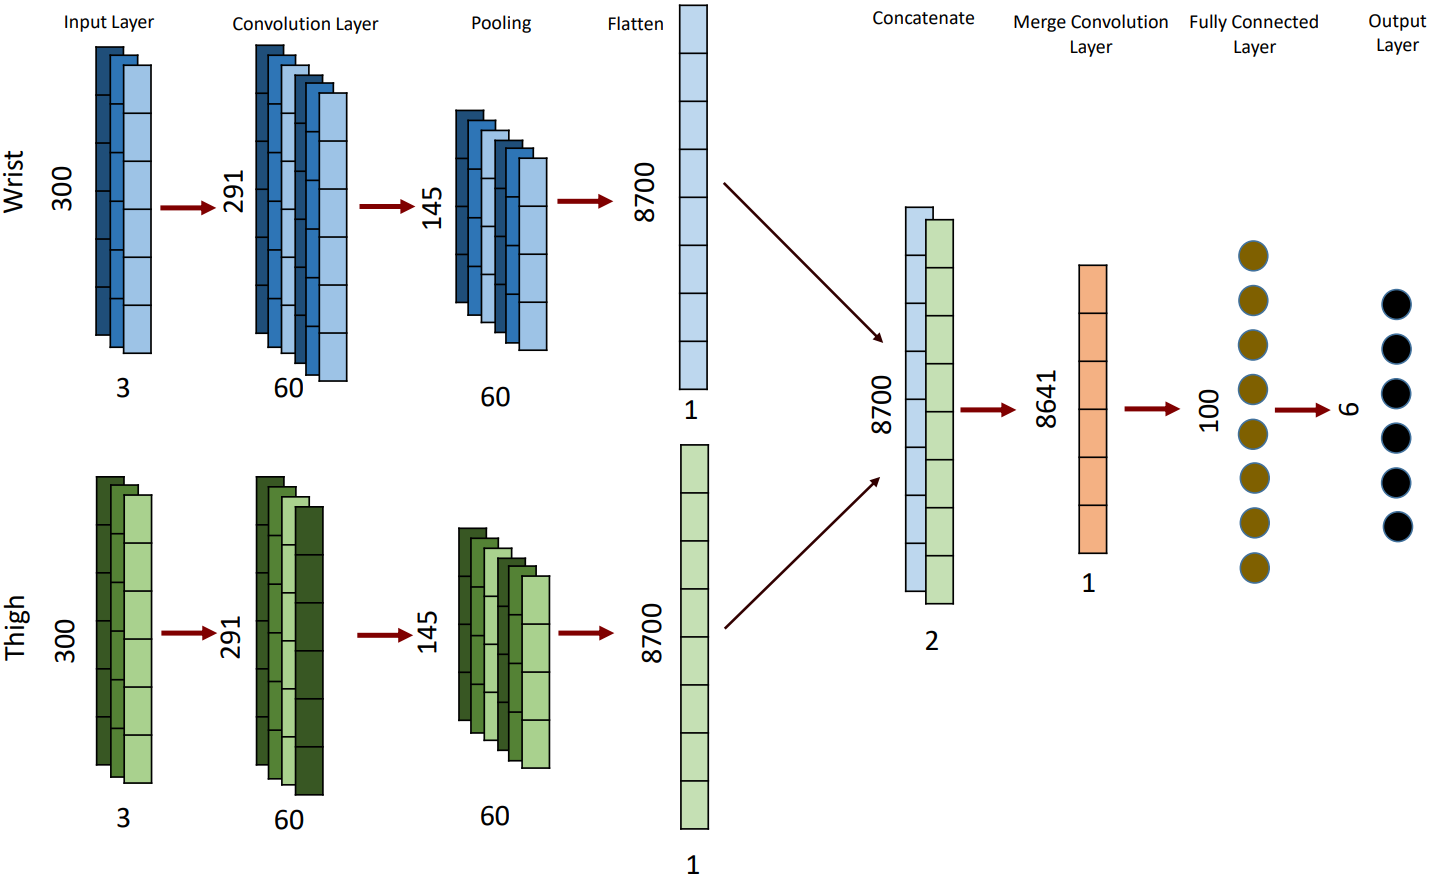
\includegraphics[width=0.5\textwidth]{concat}
\caption{Sensor Fusion Architecture with one convolution layer}
\label{fig:concat}
\end{figure}

\begin{table}[ht]
\caption{Results: Sensor Fusion architectures }
\label{table:fusion1}
\begin{center}
\begin{tabular}{|c|c|} 
  \hline
  Architecture & Test Accuracy \\
  \hline
  Wrist & 86.04738529 \\
  \hline
  Thigh & 96.44364706 \\
  \hline
  Fusion with concatenation layer & 95.94770249 \\
  \hline
\end{tabular}
\end{center}
\end{table}

We also treated each sensor axis as one input and results can be found on Table \ref{table:fusion2}. When treating each axis as one input, in the baseline model for wrist there are three individual convolutions going in to concatenation layer and in the fusion architecture there are 6 independent convolutions for each axis (Figure \ref{fig:channelconcat}).  

\begin{figure}[!ht]
\centering
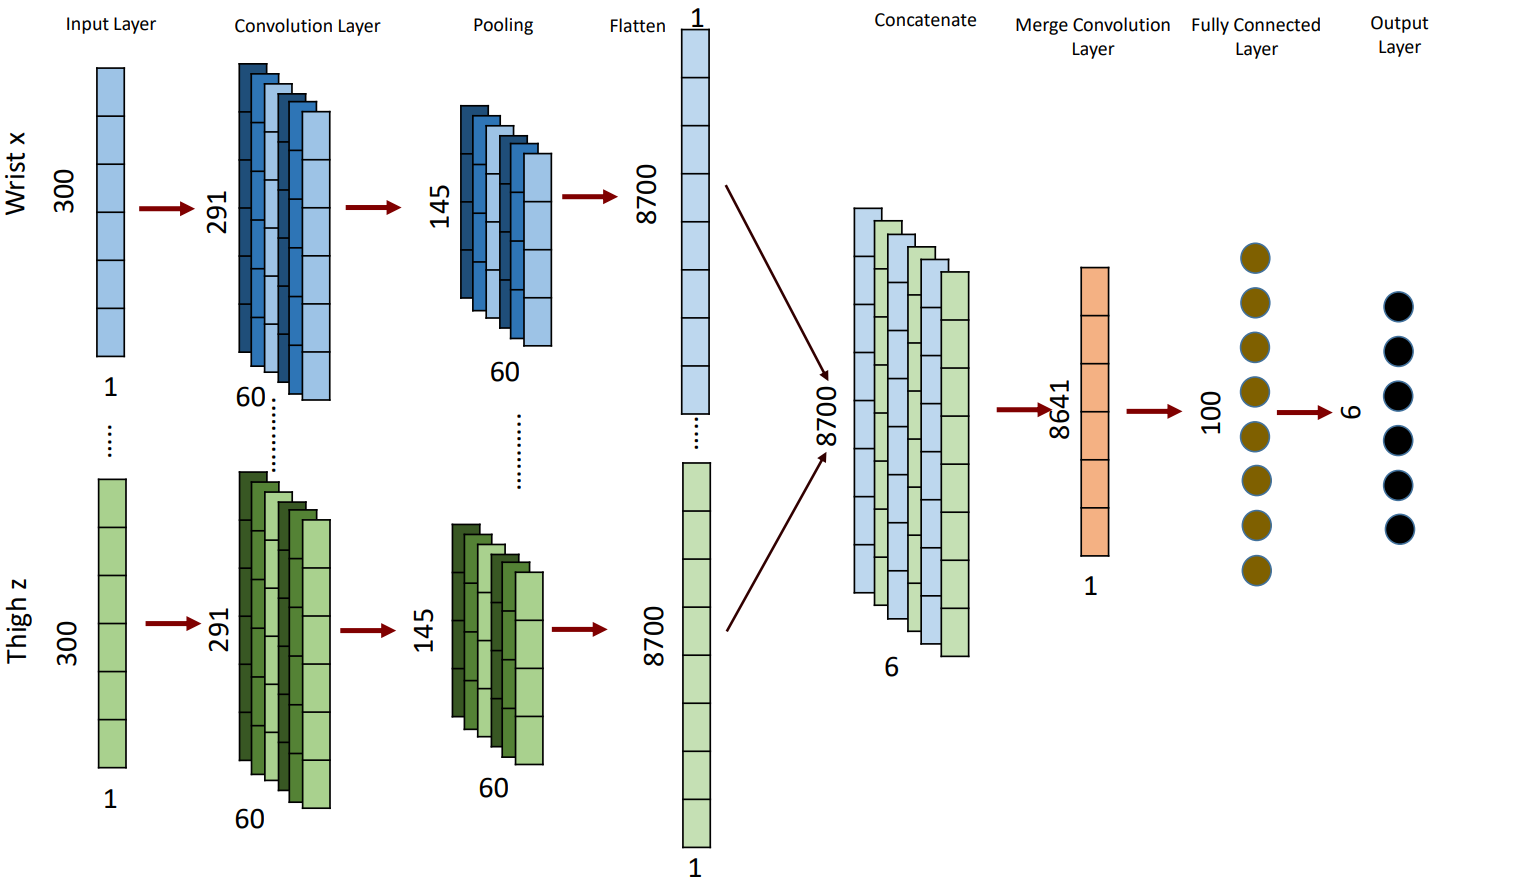
\includegraphics[width=0.5\textwidth]{conca_6}
\caption{Axis Fusion Architecture with one convolution layer}
\label{fig:channelconcat}
\end{figure}

\begin{table}[!ht]
\caption{Results: Axis Fusion architectures }
\label{table:fusion2}
\begin{center}
\begin{tabular}{|c|c|} 
  \hline
  Architecture & Test Accuracy \\
  \hline
  Wrist & 86.33278626 \\
  \hline
  Thigh & 95.99085818 \\
  \hline
  Fusion with concatenation layer & 95.96295427 \\
  \hline
\end{tabular}
\end{center}
\end{table}

From results on Table \ref{table:fusion2} we can conclude treating accelerometer data as different channels or different convolutions does not make a significant difference in performance. More importantly we can see, fusion of wrist and thigh accelerometer data does not improve overall performance of thigh accelerometer data classification.

\section*{Privileged Learning}
Next we explore opportunities of improving wrist performance with thigh data. We have already concluded that wrist is a noisy source of data (section \ref{sec:old}), but wrist is a non intrusive and familiar place to wear a sensor compared to thigh. We want to see if training a model with wrist and thigh data can make a model learn to make better decisions with just wrist data. 

We explore Privileged Learning concept with above purpose. Curriculum Learning was adapted from \citeasnoun{havaei2016hemis} to make the fusion architecture more robust to not having thigh data at test time. The curriculum strategy is we gradually decrease the number of thigh instances the model sees during 100 epochs of training. We try different drop patterns as shown in Figure\ref{fig:CLdrop} and their performance is shown in Figure \ref{fig:CLresult}

\begin{figure}[!ht]
\centering
\begin{subfigure}{.5\textwidth}
  	\centering
  	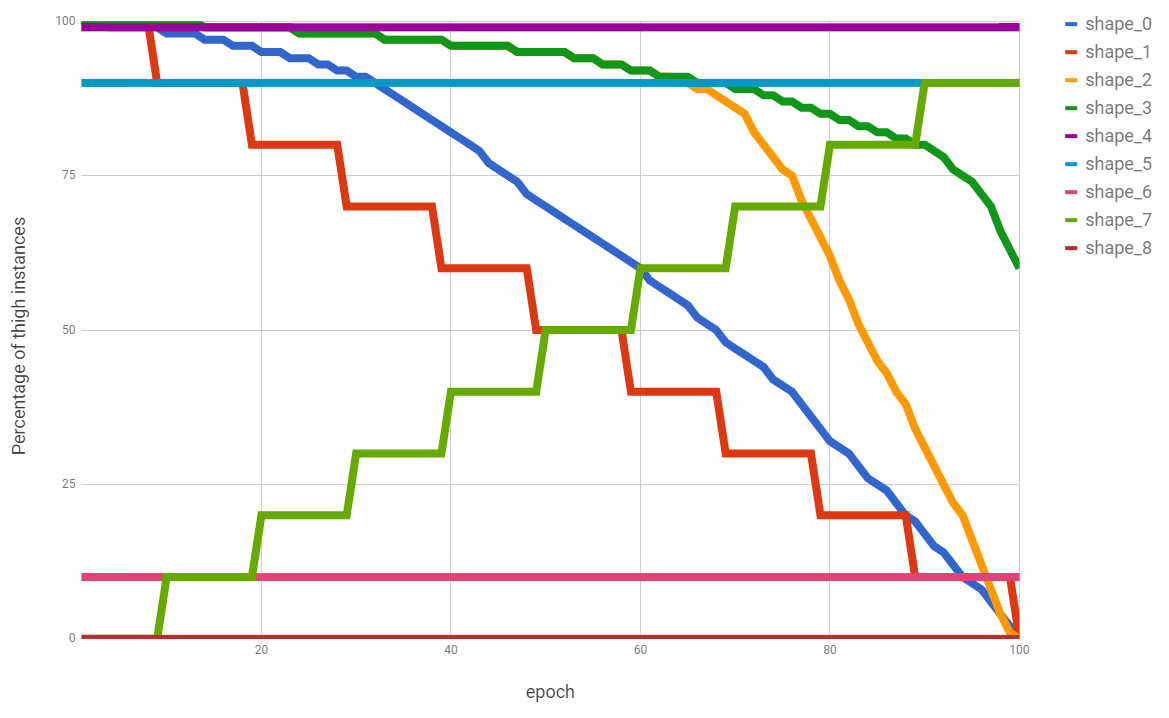
\includegraphics[width=0.8\textwidth]{curr_shapes}
	\caption{Thigh instances drop patterns}
	\label{fig:CLdrop}
\end{subfigure}%
\begin{subfigure}{.5\textwidth}
  	\centering
	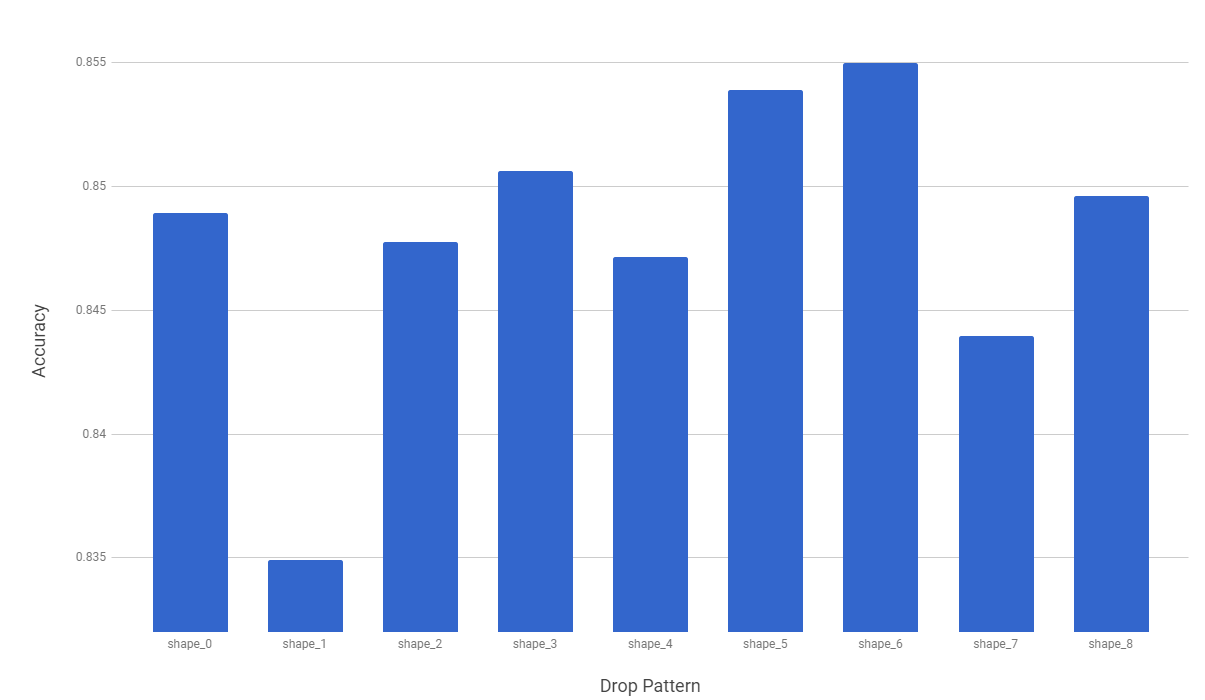
\includegraphics[width=0.8\textwidth]{curr_data}
	\caption{Results}
	\label{fig:CLresult}
\end{subfigure}
\caption{Curriculum Learning Strategies}
\label{fig:test}
\end{figure}

We can observer that dropping thigh 100 percept at all epochs during training provide significantly close performance to having thigh data. Therefore we conclude that wrist and thigh accelerometer data does not improve each-other. 

\clearpage


\section{Vitae Personal Development Planner}
\label{appendix:vitae}
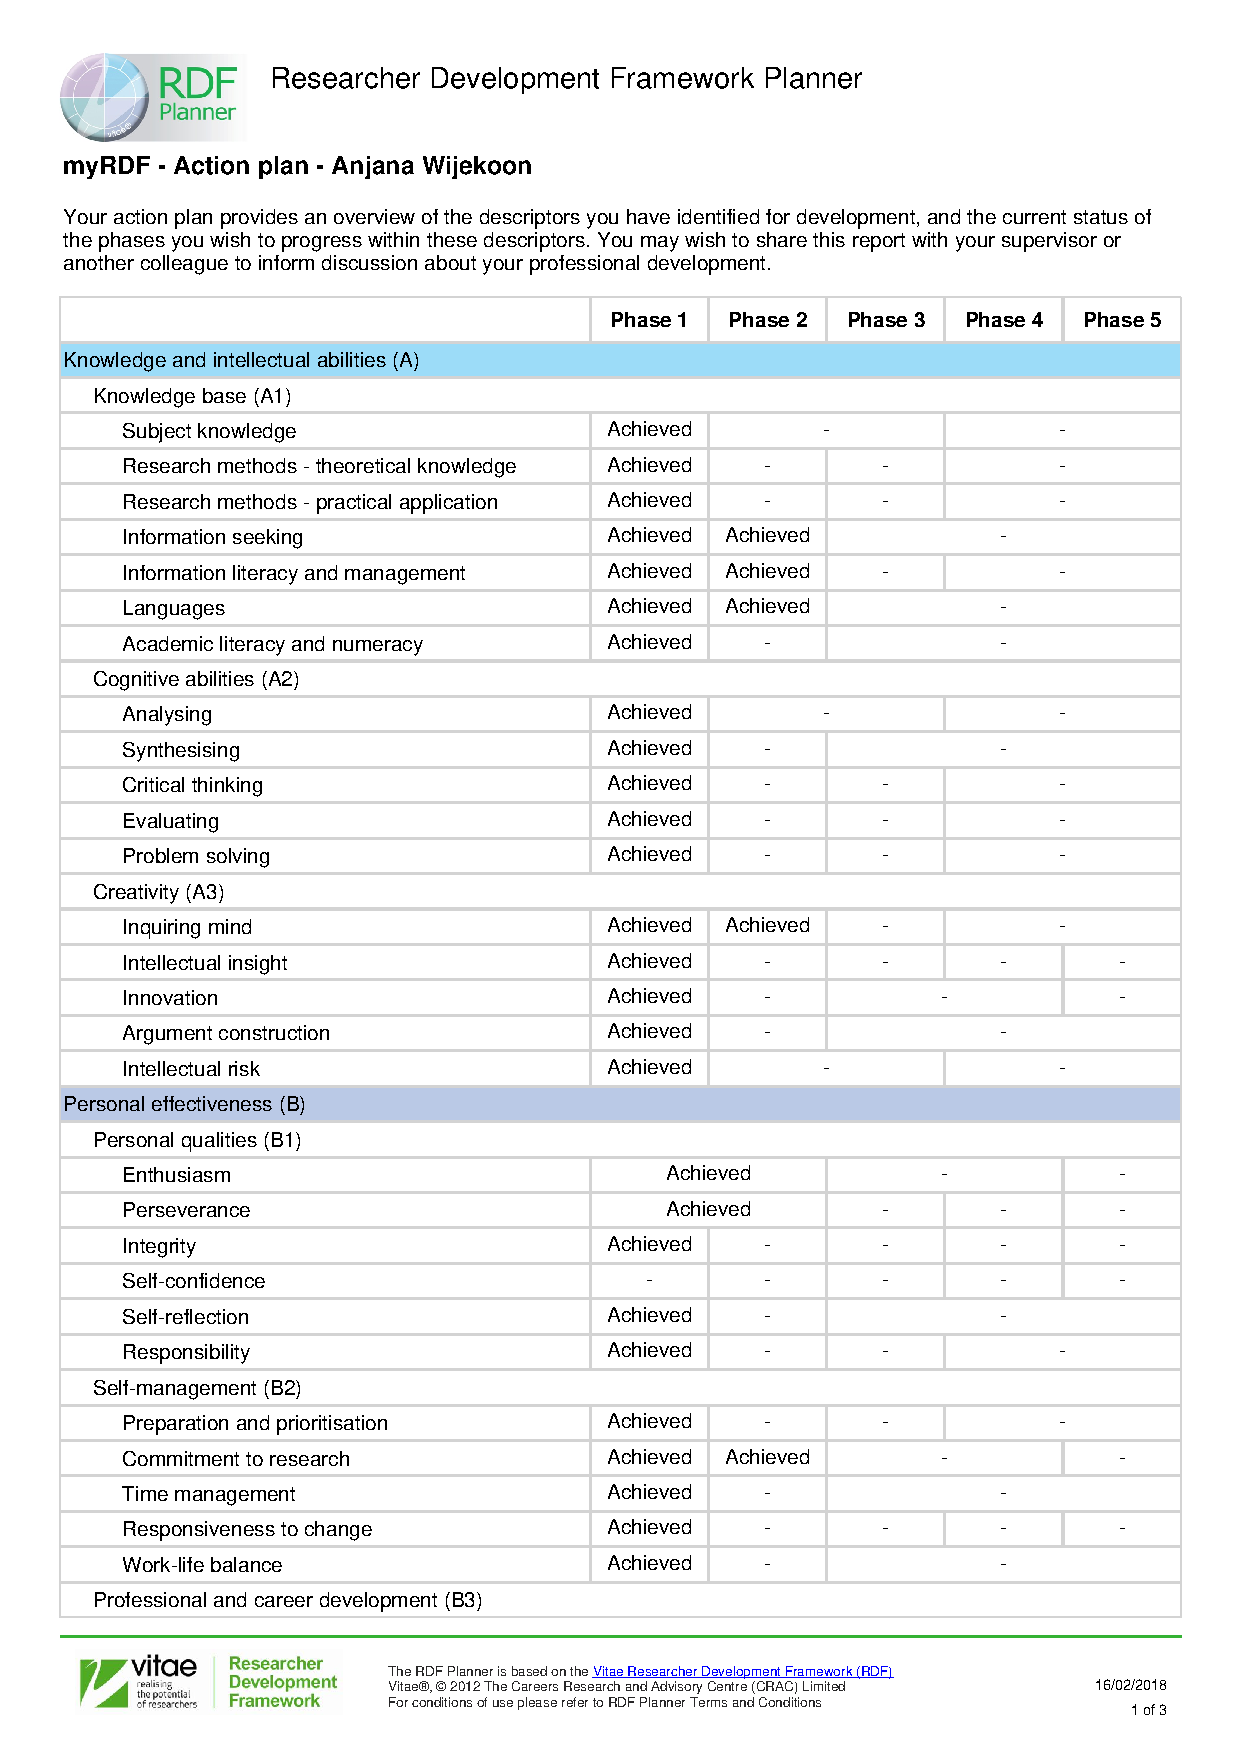
\includepdf[pages={1-3}]{misc/actionplan.pdf}

\section{Project Ethical Review Outcome}
\label{appendix:ethics}
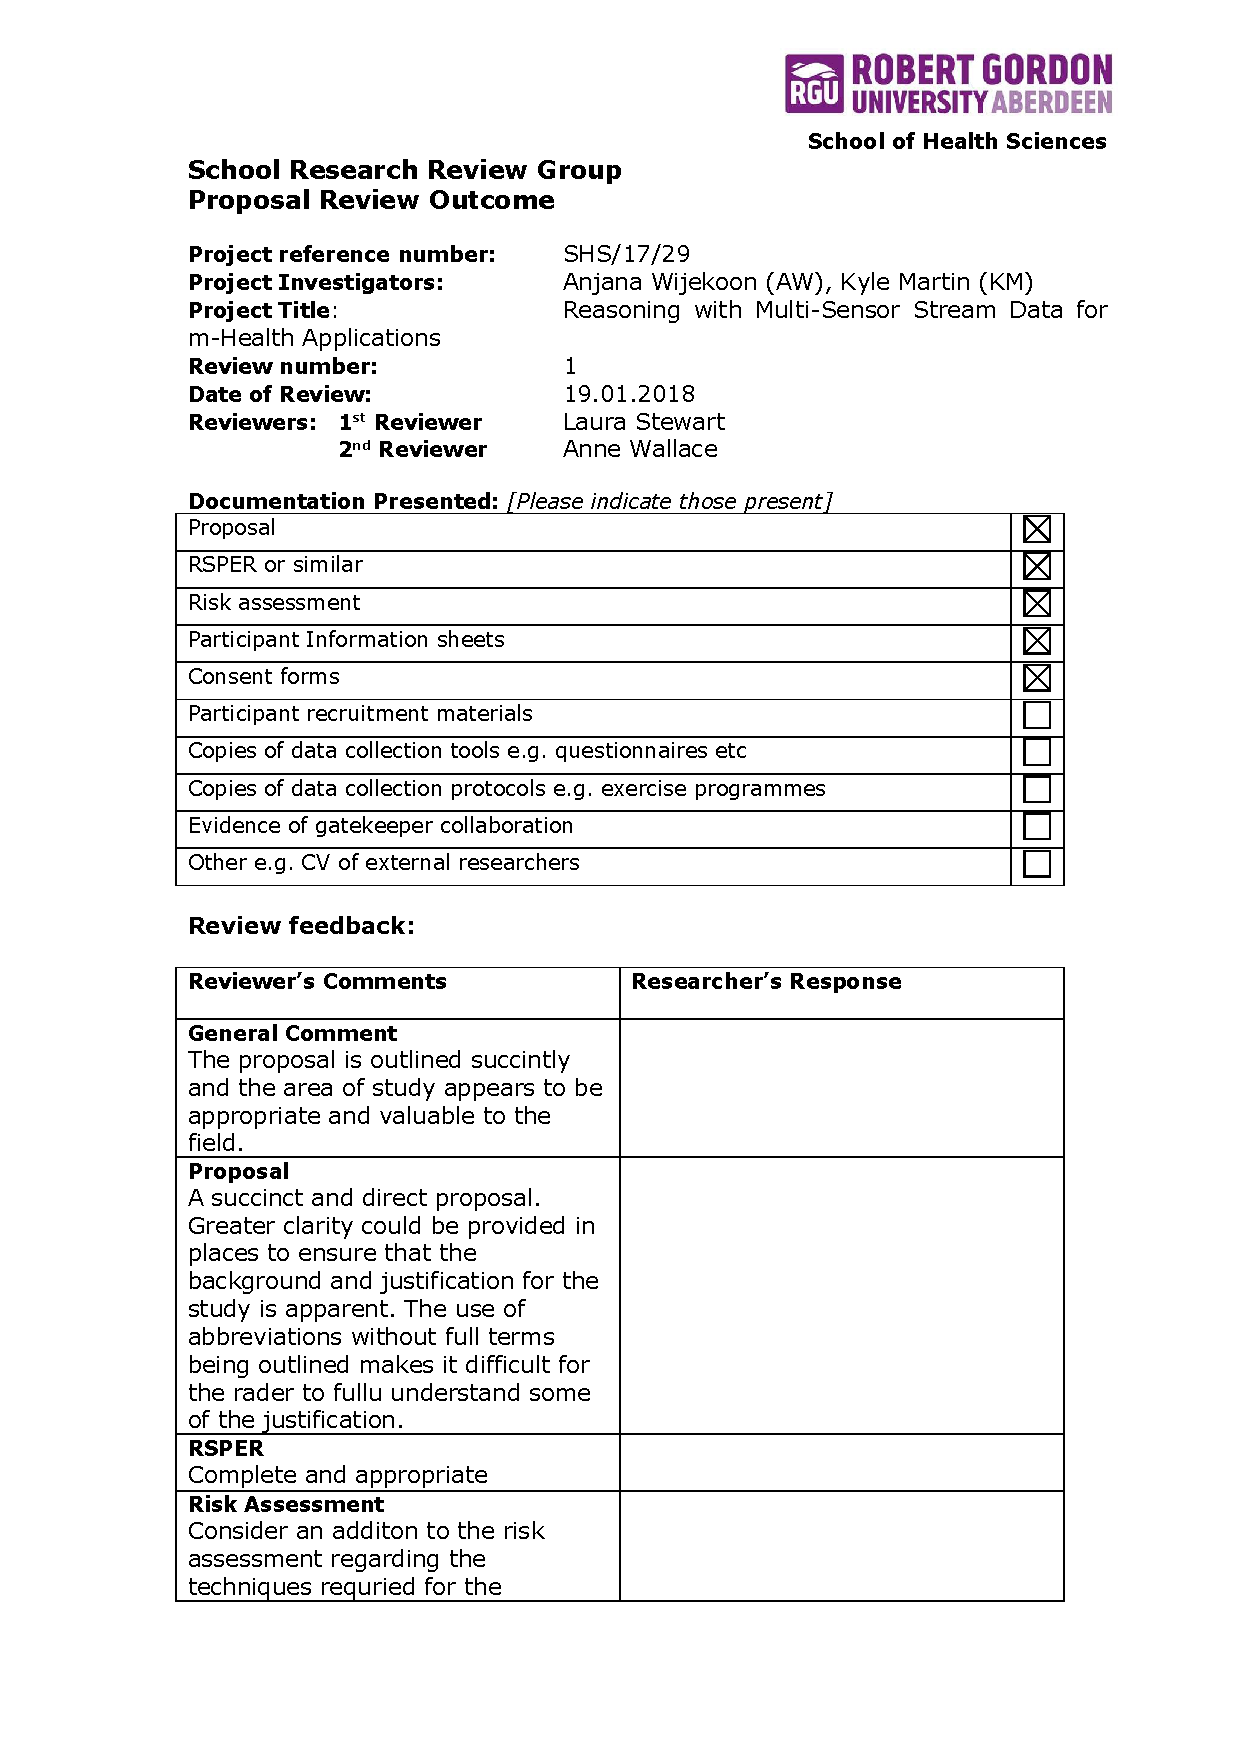
\includepdf[pages={1-3}]{misc/ethics_outcome.pdf}

\end{appendices}

\end{document}
